\part{Persistence, Consolidation, and Transformation}

\chapter{Encoding as the Creation of Recoverable Constraints}\label{ch:encoding}

Encoding is treated here as an operation that changes the set of future states that can be recovered from partial cues, not as the deposit of a copy. A history $h$ leaves a memory state $E(h)$, and what matters about that state is the set of reconstructions it makes available under a family of cues and contexts. Recoverability must therefore be defined relative to such a family, since a trace that no admissible cue can elicit is, for practical purposes, absent, and a trace that many cues can elicit is robust.

\begin{definition}[Recoverability]\label{def:recov}
Fix a cue family $Q$, a context family $\mathcal Z_0$, a target recollection function $T:\Hist\times\Cues\to\Recs$, a tolerance $\delta\ge0$, and a metric $d$ on $\Recs$. A history $h$ is $(Q,\mathcal Z_0,\delta)$-recoverable from the memory state $m$ if
\begin{equation}
\sup_{c\in Q,\,z\in\mathcal Z_0}d\bigl(\Eph(m,c,z),T(h,c)\bigr)\le\delta.
\end{equation}
It is cue-wise recoverable at $(c,z)$ if the inequality holds at that single pair.
\end{definition}

The definition makes explicit that storage of a trace does not guarantee recollection. In the softmax memory of Chapter~\ref{ch:attractor}, a trace $m_1$ among $P$ stored traces is recoverable to within $2\varepsilon$ at a cue only if the cue gives it a margin $\Delta$ over every competitor with $\Delta\ge\beta^{-1}\log\bigl((P-1)/\varepsilon\bigr)$ (Proposition~\ref{prop:basin}), and for cues orthogonal to all traces the weights are uniform and the reconstruction is the centroid of the store, from which no individual trace can be read. Adding traces raises the required margin logarithmically in $P$, which is a precise sense in which each new encoding changes the recoverability of the old ones without altering them. Conversely, a well-chosen encoding can create recoverability that did not exist: writing a trace that links a previously inaccessible content to a cue that is commonly available enlarges the recoverable set for that content without touching the content itself. The monograph accordingly describes the encoding stage by its effect on the recoverable set, and it requires of any encoding rule a statement of the cue and context families for which it intends to create recoverability.

\chapter{Consolidation and Multiscale Memory}\label{ch:consolidation}

A single store with a single timescale cannot be both plastic enough to absorb new episodes quickly and stable enough to retain old structure without interference, and the standard resolution is a division of labor among systems with different rates, in which fast learning of specific episodes is combined with slow integration of shared structure through repeated, interleaved replay \cite{mcclelland1995}. Mem8 adopts a layered form of this division. Transient activation, the fields and phases of Part~III, lives on timescales of milliseconds to seconds and is not itself persistent. A fast store holds recent traces with high fidelity and orthogonalized, pattern-separated codes, together with the full provenance of each. A slow store holds overlapping distributed codes that capture regularities across many episodes and supports semantic completion, and it is updated by replay of traces from the fast store at a small learning rate. Episode-specific provenance remains in the ledger of Chapter~\ref{ch:provenance} and is not folded into the slow store, so that consolidation changes where a content is accessible from without changing the record of where it came from.

The dynamics of transfer admit a closed form in the linear case. Let $m_f(t)$ be the strength of a trace in the fast store and $m_s(t)$ its strength in the slow store, with the fast store decaying at rate $\gamma$, replay transferring strength to the slow store at rate $\kappa$, and the slow store decaying at rate $\delta$:
\begin{equation}\label{eq:twostore}
\dot m_f=-(\gamma+\kappa)m_f,\qquad \dot m_s=\kappa m_f-\delta m_s.
\end{equation}

\begin{proposition}[Two-store solution]\label{prop:twostore}
With $a=\gamma+\kappa\ne\delta$ and initial condition $m_f(0)=m_0$, $m_s(0)=0$, the solution is
\begin{equation}
m_f(t)=m_0e^{-at},\qquad m_s(t)=\frac{\kappa\,m_0}{a-\delta}\bigl(e^{-\delta t}-e^{-at}\bigr).
\end{equation}
If $a>\delta$, the slow-store strength increases to a maximum at $t^\star=\ln(a/\delta)/(a-\delta)$ and then decays at the slow rate $\delta$.
\end{proposition}

\begin{proof}
The first equation integrates directly. For the second, multiply by $e^{\delta t}$ to obtain $\frac d{dt}(e^{\delta t}m_s)=\kappa m_0e^{-(a-\delta)t}$, integrate from zero, and rearrange. Differentiating,
\begin{equation*}
\dot m_s=\frac{\kappa m_0}{a-\delta}\bigl(ae^{-at}-\delta e^{-\delta t}\bigr),
\end{equation*}
and setting this to zero gives $ae^{-at}=\delta e^{-\delta t}$, hence $e^{(a-\delta)t}=a/\delta$.
\end{proof}

The shape is the one that systems consolidation requires: the fast-store strength falls quickly, the slow-store strength rises and persists, and the time of its maximum is controlled by the ratio of the rates. Total accessibility is the sum of the two contributions weighted by their access costs, which is why a trace that has been consolidated can be cheaper to reconstruct even when its total strength is lower. Replay in this architecture is not a literal recapitulation: it is the sampling of traces from the fast store with probability that depends on their recency, their prediction error, and their importance, followed by a small gradient or Hebbian update of the slow store, and the interleaving of old and new samples is what prevents the new material from overwriting the old, which is the catastrophic interference that sequential training would produce. Stability under continual learning is stated as an open problem in Chapter~\ref{ch:open}.

Figure~\ref{fig:twostore} plots the solution of the two-store system. The transfer from the fast to the slow store produces the characteristic crossing, after which the slow store carries the trace.

\begin{figure}[t]
\centering
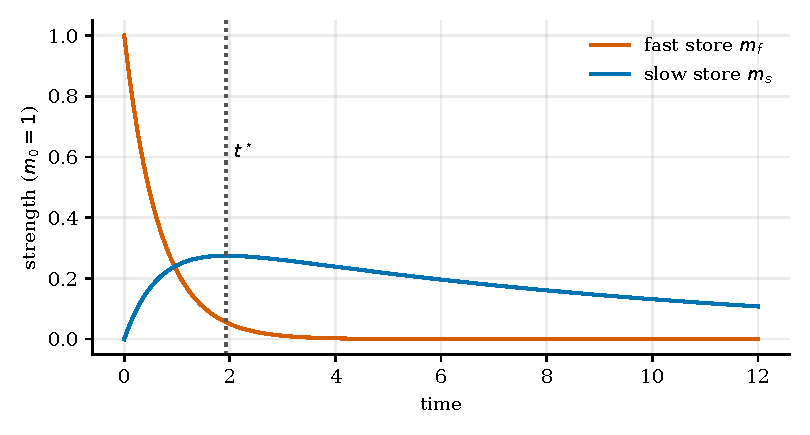
\includegraphics[width=0.85\textwidth]{figs/two_store}
\caption{Closed-form solution of Proposition~\ref{prop:twostore} for $\gamma=1$, $\kappa=0.5$, $\delta=0.1$. The slow store peaks at $t^\star$ and then decays at the slow rate. Computed by the script \texttt{figs.py} with seed 8; an illustration of the stated analytic result and not an evaluation of the architecture.}\label{fig:twostore}
\end{figure}

\section*{Worked consolidation: the two-store peak and a three-store cascade}\label{sec:cascade27}

The closed form of Proposition~\ref{prop:twostore} supports several quantities that can be computed exactly, and a cascade of more than two stores can be handled by the same method. This section gives the numbers for the parameters of Figure~\ref{fig:twostore}, treats the degenerate case that the proposition excludes, and states the cascade as a proposed extension whose proof is a partial-fraction computation.

\begin{workedex}[Peak time and transfer efficiency]\label{ex:twostore27}
Take $\gamma=1$, $\kappa=\tfrac12$ and $\delta=\tfrac1{10}$, so that $a=\tfrac32$. The slow store peaks at $t^\star=\ln(15)/1.4=\ntstar$, at which time the fast store retains $m_f(t^\star)=\nmftstar\,m_0$ and the slow store holds its maximum $m_s(t^\star)=\nmspeak\,m_0$. The maximum has the closed form
\begin{equation}
m_s(t^\star)=\frac{\kappa m_0}{a}\Bigl(\frac{\delta}{a}\Bigr)^{\delta/(a-\delta)},
\end{equation}
which follows by substituting $e^{-at^\star}=(\delta/a)\,e^{-\delta t^\star}$ and $e^{-\delta t^\star}=(\delta/a)^{\delta/(a-\delta)}$ into the solution, and it agrees with the numerical maximum to four decimals. The factor $\kappa/a=\ntransfer$ is the fraction of the initial strength that is ever transferred to the slow store, since the fast store loses strength at the total rate $a$ and the share $\kappa/a$ of that flow goes to replay; the peak is below this ceiling because the slow store is already decaying during the transfer. The consequence for design is that replay efficiency, $\kappa/(\gamma+\kappa)$, caps the slow-store strength before the slow decay rate $\delta$ is considered, so raising $\kappa$ and lowering $\gamma$ are not interchangeable with lowering $\delta$.

The case $a=\delta$ is excluded from Proposition~\ref{prop:twostore} because the denominator vanishes. Taking the limit of the solution gives $m_s(t)=\kappa m_0\,te^{-at}$, with maximum $\kappa m_0/(ae)$ at $t=1/a$. For $\gamma=\kappa=\tfrac12$ and $\delta=1$ this is $\ndegpeak\,m_0$ at $t=\ndegpeakt$, which the matrix exponential reproduces.
\end{workedex}

\begin{extension}[Cascade of $n$ stores]\label{ext:cascade27}
Let store $i$ lose strength at rate $a_i$ and pass strength to store $i+1$ at rate $k_i\le a_i$, with $m_1(0)=m_0$ and $m_i(0)=0$ for $i>1$, and let the rates $a_1,\dots,a_n$ be distinct. Then
\begin{equation}
m_n(t)=m_0\Bigl(\prod_{i=1}^{n-1}k_i\Bigr)\sum_{i=1}^n\frac{e^{-a_it}}{\prod_{j\ne i}(a_j-a_i)},
\end{equation}
and the total strength ever delivered to store $n$ is $m_0\prod_{i=1}^{n-1}k_i/a_i$.
\end{extension}

\begin{proof}
The Laplace transform of the cascade gives $\hat m_n(s)=m_0\prod_{i<n}k_i\big/\prod_{i\le n}(s+a_i)$. Since the roots $-a_i$ are simple, partial fractions give residues $1/\prod_{j\ne i}(a_j-a_i)$ at $s=-a_i$, and inversion gives the sum. For the delivered strength, store $i$ passes on the fraction $k_i/a_i$ of what it loses, and the product of these fractions along the chain is the share that reaches store $n$.
\end{proof}

The formula is the Bateman solution for a decay chain, a classical result, and it is used here for the memory interpretation and not as a new theorem.

\begin{workedex}[Three-store cascade]\label{ex:cascade27}
Take exit rates $(a_1,a_2,a_3)=(1.5,0.4,0.1)$ and transfer rates $(k_1,k_2)=(0.5,0.3)$. The second store peaks at $t=\ln(a_1/a_2)/(a_1-a_2)=\nmBpeakt$, and the third at $t=\nmDpeakt$ with strength $\nmDpeak\,m_0$, so the deeper store peaks later and lower, as the sequence of timescales requires. The strength ever delivered to the third store is $k_1k_2/(a_1a_2)=\ndelivthree\,m_0$, and the numerical integral of $a_3m_3$ over the whole time axis reproduces it, which is the conservation statement in the extension. The cascade quantifies the cost of depth: each added store multiplies the available strength by the transfer fraction $k_i/a_i$ and delays the peak, so a deep hierarchy is justified only when the recollections it serves are those that the shallow stores lose first.
\end{workedex}


\chapter{Reconsolidation and Memory Modification}\label{ch:reconsol}

The retrieval of a trace can render it labile and subject to modification before it is stabilized again, a process observed in experimental work on reconsolidation after retrieval \cite{nader2000}. In Mem8 the corresponding operation is a controlled post-retrieval update,
\begin{equation}\label{eq:reconsol}
M_{t+1}=M_t+\eta\,\mathcal U(M_t,r_t,c_t,Z_t),
\end{equation}
where $\mathcal U$ is an update direction computed from the retrieved reconstruction, the cue, and the context. Two requirements separate admissible updating from uncontrolled rewriting. The first is that the update be supported by evidence: $\mathcal U$ must depend on information that is external to the memory's own output, such as a new observation that conflicts with the retrieved reconstruction, and its magnitude must be gated by a statistic that measures the strength of that evidence. The second is that the record of what was previously stored be preserved, so that every revision can be audited and reversed.

The danger of an update that does not depend on external evidence can be stated exactly. Suppose that retrieval pulls each stored trace toward the reconstruction it helped produce, $\mathcal U_i=w_i(r-m_i)$, which is the natural form of an update driven by the memory's own output.

\begin{proposition}[Self-reinforcing distortion]\label{prop:drift}
If the update $m_i^+=m_i+\eta w_i(r-m_i)$ is applied with the reconstruction $r$ and the weights $w_i$ held fixed, then $m_i^+-r=(1-\eta w_i)(m_i-r)$. After $n$ repetitions the deviation of trace $i$ from $r$ is $(1-\eta w_i)^n(m_i-r)$, which tends to zero for every trace with $w_i>0$.
\end{proposition}

\begin{proof}
Subtract $r$ from both sides of the update. Iterating gives the stated power.
\end{proof}

Repeated retrieval under such a rule therefore collapses the traces that participate in a reconstruction onto that reconstruction, erasing the distinctions among them: what is remembered becomes what was last reconstructed, which is a formalization of the drift toward schema-consistent reproduction observed in serial reproduction studies \cite{bartlett1932}. The fixed-weights assumption makes the statement exact, and the qualitative conclusion, that distinctness is lost through self-generated updates, does not depend on it. Evidence-supported updating replaces $r$ in the update by an evidence-bearing target $e$ and gates the update by a likelihood-ratio statistic $\Lambda(e,r)$, the ratio of the probability of the evidence under the hypothesis that the retrieved reconstruction is outdated to its probability under the hypothesis that it is correct: $\mathcal U_i=g(\Lambda)\,w_i(e-m_i)$ with $g(\Lambda)=0$ below a threshold and increasing above it. A policy of this form changes a trace only when the world has told the system that it should.

The second requirement is satisfied by logging. If every update is recorded with the exact vector $\eta\,\mathcal U_s$ that was applied, then any earlier state is recoverable from a later one.

\begin{proposition}[Reversibility of logged updates]\label{prop:reverse}
If updates follow \eqref{eq:reconsol} and the ledger stores each increment $\Delta_s=\eta\,\mathcal U(M_s,r_s,c_s,Z_s)$ exactly, then $M_t=M_T-\sum_{s=t}^{T-1}\Delta_s$ for every $t\le T$.
\end{proposition}

\begin{proof}
Telescoping the recursion $M_{s+1}=M_s+\Delta_s$ from $s=t$ to $T-1$.
\end{proof}

The proposition is elementary and its consequence is the design rule of Chapter~\ref{ch:provenance}: memory modification must not silently rewrite the record of what was previously stored, and a log of increments, together with the evidence that triggered each, makes the history of a memory a first-class and recoverable object.

Figure~\ref{fig:drift} simulates the update of Proposition~\ref{prop:drift} with weights and reconstruction recomputed at every step. Traces that participate in the reconstruction collapse toward one another, while the gated update, which changes nothing without external evidence, leaves their separation intact.

\begin{figure}[t]
\centering
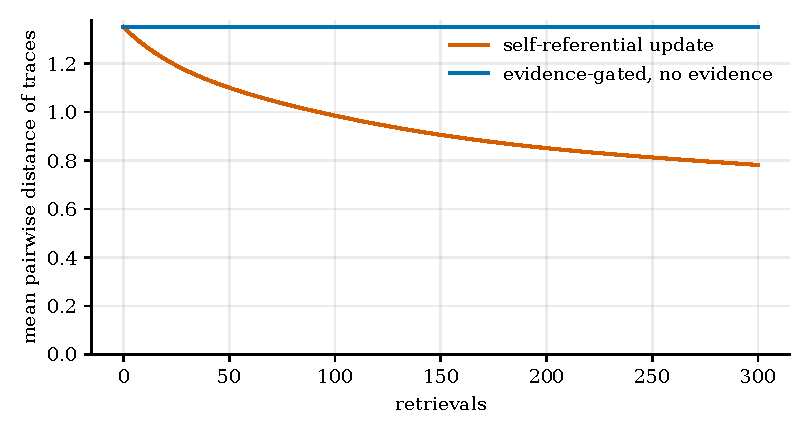
\includegraphics[width=0.85\textwidth]{figs/drift}
\caption{Mean pairwise distance among five stored traces under repeated retrieval with a self-referential update ($\eta=0.05$, $\beta=6$, fixed cue), compared with an evidence-gated update that receives no evidence. Computed by the script \texttt{figs.py} with seed 8; an illustration of the stated analytic result and not an evaluation of the architecture.}\label{fig:drift}
\end{figure}

\section*{Drift and gating: numbers and a counterexample}\label{sec:gate28}

Proposition~\ref{prop:drift} states the collapse qualitatively, and the evidence gate of the preceding discussion is a design rule whose content depends on how its statistic is computed. Two short examples fix the scale of the first and show a way in which the second can fail.

\begin{workedex}[Scale of self-reinforcing drift]\label{ex:drift28}
Hold the weight on a participating trace at $w_i=0.4$ and take the update rate $\eta=0.05$, so the contraction factor per retrieval is $1-\eta w_i=0.98$. After $n=50$ retrievals the trace retains the fraction $0.98^{50}=\ndriftfac$ of its original deviation from the reconstruction, and the deviation halves after $\nhalflifedrift$ retrievals. The collapse is therefore not a fast phenomenon at these rates: a trace that is retrieved fifty times has lost nearly two thirds of its distinctness from its neighbours, and the policy matters in the regime of heavily rehearsed material, which is the regime in which memory is least often checked against the world.
\end{workedex}

\begin{counterex}[Correlated reports pass the gate]\label{cex:gate28}
Suppose the gate opens when the likelihood ratio statistic $\Lambda$ reaches $\Lambda^\ast=10$, and that $\Lambda$ is computed as the product of the likelihood ratios of the individual reports, which is correct when the reports are conditionally independent given the hypothesis. A single report from a source that is correct with probability $0.7$ has likelihood ratio $\ell=0.7/0.3=\nellrep$. Three conditionally independent reports give $\Lambda=\ell^3=\nlamnaive>\Lambda^\ast$ and the gate opens. If the three reports are three copies of one observation, as when one source is relayed three times, the same product still gives $\nlamnaive$, whereas the correct likelihood ratio of the single underlying observation is $\nlamcopy<\Lambda^\ast$ and the gate should stay closed. The statistic is inflated by the factor $\ell^{k-1}$ for $k$ copies, which is $\ell^2=5.44$ here.
\end{counterex}

The counterexample is about the computation of the gate and not about the gate. The minimum number of conditionally independent reports of ratio $\ell$ needed to open a gate with threshold $\Lambda^\ast$ is $\lceil\ln\Lambda^\ast/\ln\ell\rceil$, which equals three for the values above because $\ln10/\ln(7/3)=\nnclusters$, and the count is meaningful only if the reports are independent. The ledger of Chapter~\ref{ch:provenance} supplies the required discipline, since every evidence record carries its source, so the gate can aggregate by source and count each at most once. This is a design constraint on the architecture and it is not a theorem about the world: sources can be correlated without being identical, and the treatment of partial dependence is left to the protocols of Part~IX.


\chapter{Forgetting, Interference, and Resource Constraints}\label{ch:forgetting}

Forgetting is defined in three ways, and the three are not equivalent. It may be a decline of recoverability, so that Definition~\ref{def:recov} fails for cue families that formerly satisfied it. It may be an increase of reconstruction cost, so that the trace remains recoverable only through a longer iteration or a more specific cue. It may be a deliberate release of a representational commitment, in which the system removes content, leaving in the ledger a record that the removal occurred. A theory that recognized only the first would treat all forgetting as loss, whereas the second and third are often the efficient and the required behavior.

The retrieval score gives amplitude decay a specific and sometimes unexpected consequence. If a stored trace of unit direction decays in amplitude as $m(t)=e^{-\gamma t}\hat m$ and the query is the aligned unit vector, then $\rho=2e^{-\gamma t}/(1+e^{-2\gamma t})=\operatorname{sech}(\gamma t)$ and by Theorem~\ref{thm:closed}
\begin{equation}\label{eq:decayscore}
S\bigl(m(t),\hat m\bigr)=\frac{\operatorname{sech}(\gamma t)}{2}\bigl(1+\operatorname{sech}(\gamma t)\bigr),
\end{equation}
which falls monotonically from one at $t=0$ toward zero, whereas the cosine of the same pair does not change with amplitude at all. Under the resonance score an older, weaker trace is therefore penalized relative to a newer one of equal alignment, producing a recency preference as a direct consequence of the energy-balance factor and without any dedicated mechanism. Whether this preference is desirable is a matter of policy: it is appropriate when recency predicts relevance and inappropriate when the old trace is the better evidence. The corollary for architecture is that amplitude must be treated as a managed quantity, either normalized at write time and given an explicit age feature, or allowed to carry age deliberately, and that the choice must be recorded as part of the specification.

Resource-sensitive forgetting is the policy of choosing which traces to release when a budget is binding. The comparison with indiscriminate temporal decay is clean in the simplest case.

\begin{proposition}[Optimal retention under a budget]\label{prop:retention}
Suppose each of $N$ items will be queried in the future independently with probabilities $p_1,\dots,p_N$, a query for a retained item succeeds and a query for a released item fails, and at most $B$ items can be retained. The retention set that maximizes the expected number of successful queries is the set of $B$ items with the largest $p_i$. A policy that retains the $B$ youngest items attains the optimum if and only if the access probability is nonincreasing in age, in the sense that the youngest $B$ items are among the $B$ largest $p_i$.
\end{proposition}

\begin{proof}
The expected number of successes is $\sum_{i\in R}p_i$ over the retained set $R$, which is maximized under the cardinality constraint by selecting the $B$ largest values. The age-based policy selects the $B$ youngest, which coincides with this set exactly when those items carry the $B$ largest probabilities.
\end{proof}

The proposition does not say that decay is wrong; it says that decay is optimal precisely when age is a sufficient statistic for future access, and that where other predictors are available, such as the number of distinct contexts in which an item was previously retrieved, the provenance of the item, or its dependence by other retained items, a better policy exists. The monograph compares learned and rule-based retention policies against age-based decay in Chapter~\ref{ch:scaling} at matched budgets, and deliberate release is implemented by tombstone records that remove the content while preserving in the ledger the facts that the trace existed and that it was released, with the content removed in full when erasure is required.

\section*{Retention and recency: a counterexample and a closed form}\label{sec:retain29}

\begin{counterex}[Youngest-first retention is not optimal]\label{cex:retain29}
Let six items, listed from youngest to oldest, have future access probabilities $(0.10,0.50,0.05,0.30,0.02,0.40)$ and let the budget be $B=3$. The age-based policy retains the three youngest and obtains an expected $\nretyoung$ successful queries, while the optimal policy of Proposition~\ref{prop:retention} retains the items with probabilities $0.50$, $0.40$ and $0.30$ and obtains $\nretopt$. The regret is $\nregret$ expected queries, nearly half of the optimum. The example is built so that age is a poor predictor, and the proposition says exactly when this happens: the age policy is optimal if and only if the youngest $B$ items are the $B$ most probable. Whether any real memory has access probabilities of this form is a matter of measurement, and the example makes no claim about it.
\end{counterex}

\begin{workedex}[Recency from the energy-balance factor]\label{ex:recency29}
For a trace decaying as $m(t)=e^{-\gamma t}\hat m$ and an aligned unit query, equation~\eqref{eq:decayscore} gives scores that depend only on $\gamma t$. At $\gamma t=1$ one has $\operatorname{sech}(1)=\nrhoB$ and $S=\nSdecayB$, at $\gamma t=2$ one has $\nrhotwo$ and $\nSdectwo$, and at $\gamma t=3$ one has $\nrhothree$ and $\nSdecthree$, while the cosine of the same pair stays at one throughout. The score falls to one half when $\rho(1+\rho)=1$, that is, when $\rho$ is the reciprocal of the golden ratio, and the corresponding age is $\gamma t=\operatorname{arcosh}\varphi=\ngtheigh$. The resonance score therefore imposes a definite recency scale on a store in which amplitude decays, and the scale is set by $\gamma$ alone: a trace loses half its score at about one decay time, regardless of its alignment. This is a consequence of the closed form of Theorem~\ref{thm:closed} and not a finding about memory.
\end{workedex}


\chapter{Memory Compression and Future Admissibility}\label{ch:compression}

Compression of a store is acceptable not when it reduces storage by some factor but when it preserves what future reconstruction needs. Let $\mathcal Q$ be a family of admissible future queries, let $C$ be a compression map applied to the memory state, and let $d$ be a distance on reconstructions. The objective is a bound
\begin{equation}\label{eq:compbound}
\sup_{q\in\mathcal Q}d\bigl(\Eph(q,M),\Eph(q,C(M))\bigr)\le\varepsilon,
\end{equation}
which ties the permitted loss directly to preserved reconstructive capacity and not to a storage criterion. Two limiting cases clarify the content of the bound. If $C$ factors through the quotient by recollective equivalence, in the sense that $C(M)$ determines the class of $M$ under $\sim_{\mathcal Q}$, then the supremum is zero for any $\varepsilon\ge0$, and the compression is lossless with respect to $\mathcal Q$; this is the sufficiency theorem of Chapter~\ref{ch:ident} in the language of compression. At the other extreme, a compression that discards any distinction that some query in $\mathcal Q$ depends on has a strictly positive supremum, whatever its storage savings.

For the softmax reconstruction the bound can be made explicit.

\begin{proposition}[Distortion bound for the softmax readout]\label{prop:distort}
Let $M=(m_1,\dots,m_P)$ and $M'=(m_1',\dots,m_P')$ be stores with $\norm{m_i},\norm{m_i'}\le1$ and $\max_i\norm{m_i-m_i'}\le\delta$, and let $F_M(c)=\sum_iw_i(c)m_i$ with $w=\softmax(\beta\ip{m_i}{c})$ for a query $c$ with $\norm c\le1$. Then $\norm{F_M(c)-F_{M'}(c)}\le(1+2\beta)\delta$.
\end{proposition}

\begin{proof}
The scores differ by at most $\delta$ in each coordinate, since $|\ip{m_i-m_i'}{c}|\le\delta$. The derivative of the softmax is $\beta(\operatorname{diag}(w)-ww^\top)$, and for a perturbation $v$ with $\norm v_\infty\le\delta$ its image has $\ell_1$ norm at most $\beta\sum_iw_i|v_i-\bar v|\le2\beta\delta$, with $\bar v=\sum_jw_jv_j$. Integrating along the segment between the two score vectors gives $\norm{w-w'}_1\le2\beta\delta$. Then $\norm{F_M-F_{M'}}\le\norm{\sum_i(w_i-w_i')m_i}+\norm{\sum_iw_i'(m_i-m_i')}\le2\beta\delta+\delta$.
\end{proof}

The bound shows that the distortion permitted to each trace is inversely proportional to $1+2\beta$, so sharper selection, which is useful for discrimination, makes the readout more sensitive to compression error, and therefore trades against compressibility. For the storage cost of achieving a given per-trace distortion, the rate--distortion function of a Gaussian source with independent components of variance $\sigma^2$ under squared error is $R(D)=\frac12\log_2(\sigma^2/D)$ bits per component for $D<\sigma^2$ \cite{cover2006}. For a trace with $d$ real components and a target distortion $\norm{m-m'}^2\le\delta^2$, with $D=\delta^2/d$ per component, this gives
\begin{equation}
R(\delta)=\frac d2\log_2\frac{d\sigma^2}{\delta^2}\ \text{bits per trace},\qquad\delta^2<d\sigma^2,
\end{equation}
as a lower bound on the representation size under this source model, and the budget of Proposition~\ref{prop:distort} then fixes $\delta$ from the desired reconstruction accuracy. For low-rank compression of a store matrix, the Eckart--Young theorem states that the best rank-$k$ approximation in the Frobenius norm has error $\bigl(\sum_{j>k}\sigma_j^2\bigr)^{1/2}$ in terms of the singular values of the store, and each trace is perturbed by at most that amount, so the singular spectrum of the store determines how far it can be compressed under a given $\varepsilon$ \cite{eckart1936}. These are bounds under stated source models, and the monograph treats the sufficiency-based compression, which discards by equivalence class and not by magnitude, as the quantity of primary interest, since it can compress by much more than any magnitude-based method when most of the stored structure is irrelevant to the admissible queries.

\section*{How tight is the distortion bound?}\label{sec:distort30}

Proposition~\ref{prop:distort} bounds the change of the softmax readout under a perturbation of the store by $(1+2\beta)\delta$. Two questions about this bound can be answered by computation: how loose it is on typical stores, and whether its linear growth in $\beta$ is an artifact of the proof.

\begin{workedex}[Looseness on random stores]\label{ex:looseness30}
In 300 random stores with $3\le P\le19$ traces in dimensions $4$ to $29$, inverse temperatures drawn uniformly from $[0.5,15]$, perturbations of size up to $0.1$, and five random cues each, the largest observed ratio of $\norm{F_M(c)-F_{M'}(c)}$ to $(1+2\beta)\delta$ was $\ncompratio$. The bound therefore held in every instance and was typically loose by a factor of several, as expected of a worst-case bound on random data. This is an algebraic check of the proposition, with a fixed seed, and it is not a statement about any memory system.
\end{workedex}

\begin{extension}[The linear dependence on $\beta$ is necessary]\label{ext:sharp30}
There are stores and queries for which $\norm{F_M(c)-F_{M'}(c)}\ge\tfrac{\sqrt3}{2}\tanh(\beta\delta/2)$ with $\max_i\norm{m_i-m_i'}=\delta$. Consequently $\sup\norm{F_M-F_{M'}}/\delta\ge\tfrac{\sqrt3}{4}\beta(1+o(1))$ as $\delta\to0$ for each fixed $\beta$, and the factor $1+2\beta$ in Proposition~\ref{prop:distort} cannot be replaced by any function that is $o(\beta)$.
\end{extension}

\begin{proof}
In $\R^2$ take the cue $c=(1,0)$ and the traces $m_1=(\tfrac12,\tfrac{\sqrt3}2)$ and $m_2=(\tfrac12,-\tfrac{\sqrt3}2)$, which are unit vectors with equal scores $\tfrac12$ against $c$. Perturb $m_1$ to $m_1'=m_1+\delta c$. Then $w_1'=1/(1+e^{-\beta\delta})$ and $w_2'=1-w_1'$, and $F_{M'}-F_M$ has second coordinate $\tfrac{\sqrt3}2(w_1'-w_2')=\tfrac{\sqrt3}2\tanh(\beta\delta/2)$, since the unperturbed weights are equal and the second coordinates of $m_1$ and $m_2$ are opposite. The norm is at least the absolute value of this coordinate, and $\tanh(x)\ge x(1+o(1))$ as $x\to0$.
\end{proof}

For $\beta=10$ and $\delta=0.01$ the exact ratio $\norm{F_M-F_{M'}}/\delta$ is $\nsharpvalBA$ against the proposition's bound of $21$, and for $\beta=40$ and $\delta=0.0025$ it is $\nsharpvalEA$ against $81$. The ratios to the bound are $\nsharpBA$ and $\nsharpEA$, so the bound is tight up to a factor of about five in this family and the proof's linear dependence on $\beta$ reflects a real sensitivity. A store sharp enough for selective recall in the sense of Chapter~\ref{ch:stability} is therefore a store whose readout is correspondingly sensitive to quantization or pruning of the traces, and the compression budget $\varepsilon$ of \eqref{eq:compbound} must be spent at a rate that scales inversely with $\beta$.

\section*{Synthesis of Part~VI}\label{sec:synth6}

The examples of this part share a structure: each chapter fixes a rate or a sensitivity, and the examples show that the rate is controlled by a small number of quantities that can be read off the model. In consolidation the controlling quantities are the exit rates and transfer fractions, which determine both when the deeper store peaks and how much strength it ever receives (Extension~\ref{ext:cascade27}), so that the delivered fraction $k_1k_2/(a_1a_2)=\ndelivthree$ is fixed by the rates before any content is considered. In reconsolidation the controlling quantity is the contraction factor $1-\eta w_i$ of the self-referential update, which sets the half-life of distinctness at $\nhalflifedrift$ retrievals for the example rates, together with the independence of the evidence that opens the gate (Counterexample~\ref{cex:gate28}). In forgetting it is the match between the retention rule and the access probabilities (Counterexample~\ref{cex:retain29}) and the recency scale $\operatorname{arcosh}\varphi$ that the energy-balance factor builds in (Worked Example~\ref{ex:recency29}). In compression it is the product of the inverse temperature and the perturbation size (Extension~\ref{ext:sharp30}).

The results connect through the temperature and through the sufficiency criterion. A store that is sharp enough for selective retrieval, with $\beta$ above the thresholds of Chapter~\ref{ch:stability}, is also a store that amplifies perturbations linearly in $\beta$, so the compression that consolidation performs when it moves strength into a slower, more overlapping store has a cost that grows with the selectivity it is meant to support. Reconsolidation determines whether the distinctions the slow store receives are distinctions of the world or of the system's own earlier reconstructions, and the gate computation determines whether the evidence for a revision is counted once or several times. Forgetting then decides, under a budget, which of the surviving traces are kept, and Proposition~\ref{prop:retention} is the statement that this decision should be made on predicted access and not on age unless age is a sufficient statistic. All four operations are changes to the stored state, and the criterion of Theorem~\ref{thm:suff} applies after each of them: an operation is admissible with respect to the committed recollections only if it does not merge histories that those recollections distinguish. Part~VII makes this the organizing principle, and the viability-preserving equivalence of Extension~\ref{ext:viabequiv} is the form that principle takes when the operations are repeated.

The same caveats hold as for Part~VII. The rates are those of linear models chosen so that the solutions are in closed form, the retention probabilities and the report likelihoods are constructed to expose a logical point, and none of these numbers is an estimate of a quantity in a biological or deployed memory. The numerical statements were produced by the script \texttt{examples.py} and cross-checked against the matrix exponential or by direct simulation as noted at each example.
